\documentclass{standalone}
\usepackage{tikz}
\usetikzlibrary{patterns, positioning}


\begin{document}
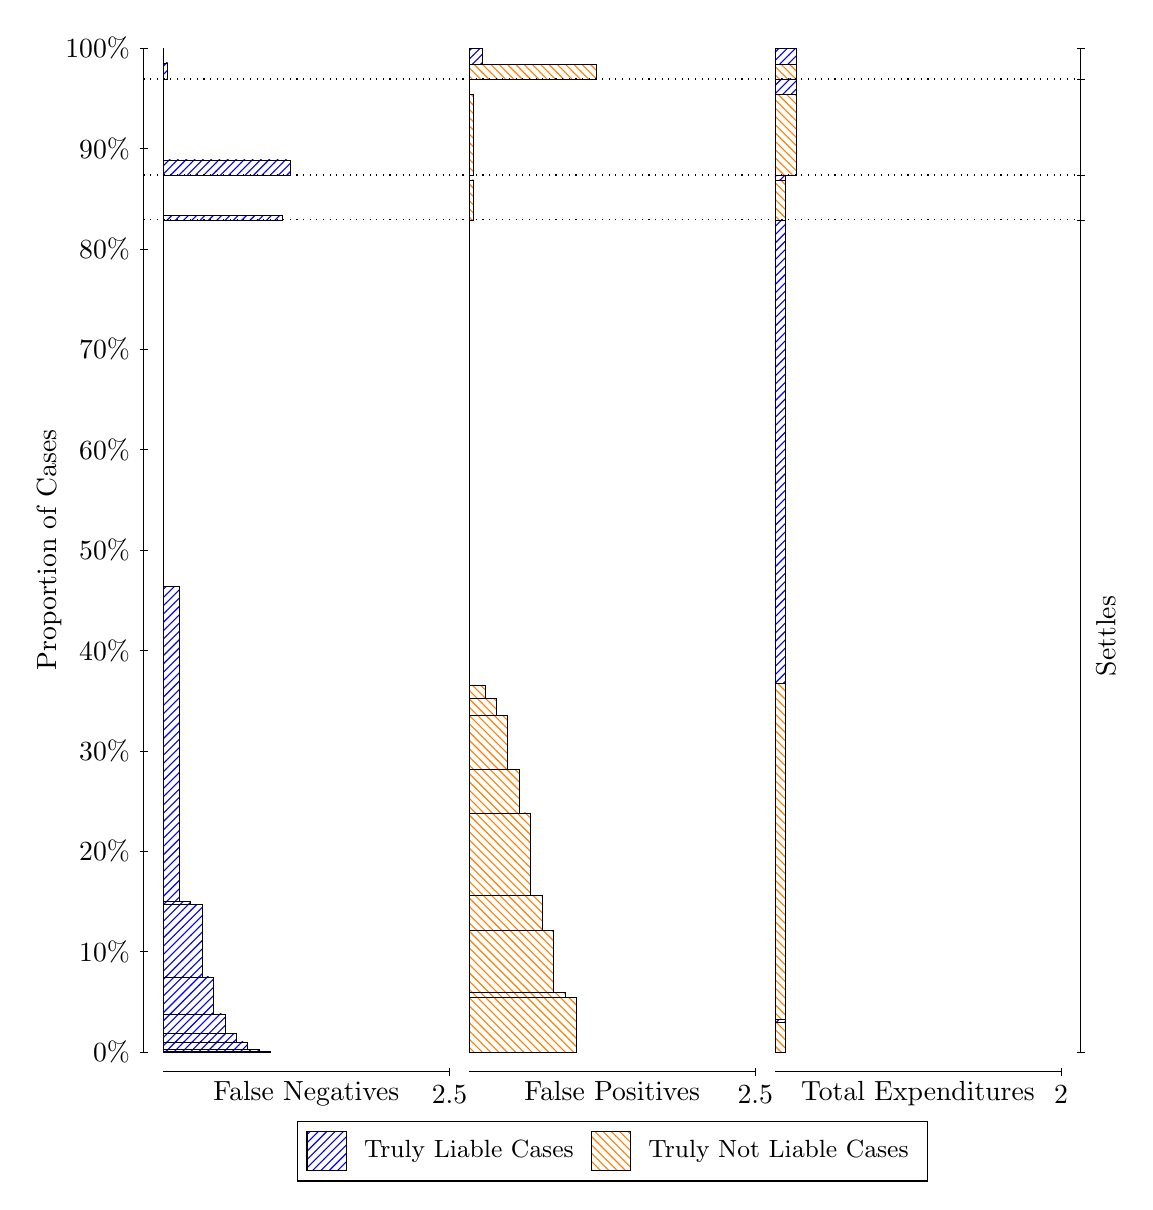
\begin{tikzpicture}
\draw[black, very thin] (1.5,1.75) -- (1.5,14.5);
\node[rotate=90, text=black, anchor=center] at (0.3, 8.125) {Proportion of Cases};
\draw[black, very thin] (1.45,1.75) -- (1.55,1.75);
\node[text=black, anchor=east] at (1.45, 1.75) {0\%};
\draw[black, very thin] (1.45,3.025) -- (1.55,3.025);
\node[text=black, anchor=east] at (1.45, 3.025) {10\%};
\draw[black, very thin] (1.45,4.3) -- (1.55,4.3);
\node[text=black, anchor=east] at (1.45, 4.3) {20\%};
\draw[black, very thin] (1.45,5.575) -- (1.55,5.575);
\node[text=black, anchor=east] at (1.45, 5.575) {30\%};
\draw[black, very thin] (1.45,6.85) -- (1.55,6.85);
\node[text=black, anchor=east] at (1.45, 6.85) {40\%};
\draw[black, very thin] (1.45,8.125) -- (1.55,8.125);
\node[text=black, anchor=east] at (1.45, 8.125) {50\%};
\draw[black, very thin] (1.45,9.4) -- (1.55,9.4);
\node[text=black, anchor=east] at (1.45, 9.4) {60\%};
\draw[black, very thin] (1.45,10.675) -- (1.55,10.675);
\node[text=black, anchor=east] at (1.45, 10.675) {70\%};
\draw[black, very thin] (1.45,11.95) -- (1.55,11.95);
\node[text=black, anchor=east] at (1.45, 11.95) {80\%};
\draw[black, very thin] (1.45,13.225) -- (1.55,13.225);
\node[text=black, anchor=east] at (1.45, 13.225) {90\%};
\draw[black, very thin] (1.45,14.5) -- (1.55,14.5);
\node[text=black, anchor=east] at (1.45, 14.5) {100\%};

\draw[black, very thin] (13.4,1.75) -- (13.4,14.5);
\draw[black, very thin] (13.35,1.75) -- (13.45,1.75);
\node[anchor=west] at (13.35, 1.75) {};
\draw[black, very thin] (13.35,12.317) -- (13.45,12.317);
\node[anchor=west] at (13.35, 12.317) {};
\draw[black, very thin] (13.35,12.887) -- (13.45,12.887);
\node[anchor=west] at (13.35, 12.887) {};
\draw[black, very thin] (13.35,14.107) -- (13.45,14.107);
\node[anchor=west] at (13.35, 14.107) {};
\draw[black, very thin] (13.35,14.5) -- (13.45,14.5);
\node[anchor=west] at (13.35, 14.5) {};

\draw[black, very thin, pattern color=blue, pattern=north east lines] (1.75,1.75) rectangle (3.1125,1.7624);
\draw[black, very thin, pattern color=blue, pattern=north east lines] (1.75,1.7624) rectangle (2.9672,1.7844);
\draw[black, very thin, pattern color=blue, pattern=north east lines] (1.75,1.7844) rectangle (2.8218,1.8793);
\draw[black, very thin, pattern color=blue, pattern=north east lines] (1.75,1.8793) rectangle (2.6765,1.9829);
\draw[black, very thin, pattern color=blue, pattern=north east lines] (1.75,1.9829) rectangle (2.5312,2.235);
\draw[black, very thin, pattern color=blue, pattern=north east lines] (1.75,2.235) rectangle (2.3858,2.7028);
\draw[black, very thin, pattern color=blue, pattern=north east lines] (1.75,2.7028) rectangle (2.2405,3.6258);
\draw[black, very thin, pattern color=blue, pattern=north east lines] (1.75,3.6258) rectangle (2.0952,3.662);
\draw[black, very thin, pattern color=blue, pattern=north east lines] (1.75,3.662) rectangle (1.9498,7.6659);
\draw[black, very thin, pattern color=orange, pattern=north west lines] (1.75,7.6659) rectangle (1.75,12.317);
\draw[black, very thin, pattern color=blue, pattern=north east lines] (1.75,12.317) rectangle (3.2578,12.379);
\draw[black, very thin, pattern color=orange, pattern=north west lines] (1.75,12.379) rectangle (1.75,12.887);
\draw[black, very thin, pattern color=blue, pattern=north east lines] (1.75,12.887) rectangle (3.3668,13.079);
\draw[black, very thin, pattern color=orange, pattern=north west lines] (1.75,13.079) rectangle (1.75,14.107);
\draw[black, very thin, pattern color=blue, pattern=north east lines] (1.75,14.107) rectangle (1.8045,14.312);
\draw[black, very thin, pattern color=orange, pattern=north west lines] (1.75,14.312) rectangle (1.75,14.5);
\draw[black, very thin, pattern color=orange, pattern=north west lines] (5.6333,1.75) rectangle (6.9958,2.4469);
\draw[black, very thin, pattern color=orange, pattern=north west lines] (5.6333,2.4469) rectangle (6.8505,2.5068);
\draw[black, very thin, pattern color=orange, pattern=north west lines] (5.6333,2.5068) rectangle (6.7052,3.292);
\draw[black, very thin, pattern color=orange, pattern=north west lines] (5.6333,3.292) rectangle (6.5598,3.7426);
\draw[black, very thin, pattern color=orange, pattern=north west lines] (5.6333,3.7426) rectangle (6.4145,4.7868);
\draw[black, very thin, pattern color=orange, pattern=north west lines] (5.6333,4.7868) rectangle (6.2692,5.3378);
\draw[black, very thin, pattern color=orange, pattern=north west lines] (5.6333,5.3378) rectangle (6.1238,6.0223);
\draw[black, very thin, pattern color=orange, pattern=north west lines] (5.6333,6.0223) rectangle (5.9785,6.2404);
\draw[black, very thin, pattern color=orange, pattern=north west lines] (5.6333,6.2404) rectangle (5.8332,6.4014);
\draw[black, very thin, pattern color=blue, pattern=north east lines] (5.6333,6.4014) rectangle (5.6333,12.317);
\draw[black, very thin, pattern color=orange, pattern=north west lines] (5.6333,12.317) rectangle (5.6878,12.825);
\draw[black, very thin, pattern color=blue, pattern=north east lines] (5.6333,12.825) rectangle (5.6333,12.887);
\draw[black, very thin, pattern color=orange, pattern=north west lines] (5.6333,12.887) rectangle (5.6878,13.915);
\draw[black, very thin, pattern color=blue, pattern=north east lines] (5.6333,13.915) rectangle (5.6333,14.107);
\draw[black, very thin, pattern color=orange, pattern=north west lines] (5.6333,14.107) rectangle (7.2502,14.295);
\draw[black, very thin, pattern color=blue, pattern=north east lines] (5.6333,14.295) rectangle (5.7968,14.5);
\draw[black, very thin, pattern color=orange, pattern=north west lines] (9.5167,1.75) rectangle (9.6529,2.1291);
\draw[black, very thin, pattern color=blue, pattern=north east lines] (9.5167,2.1291) rectangle (9.6529,2.1635);
\draw[black, very thin, pattern color=orange, pattern=north west lines] (9.5167,2.1635) rectangle (9.6529,6.4358);
\draw[black, very thin, pattern color=blue, pattern=north east lines] (9.5167,6.4358) rectangle (9.6529,12.317);
\draw[black, very thin, pattern color=orange, pattern=north west lines] (9.5167,12.317) rectangle (9.6529,12.825);
\draw[black, very thin, pattern color=blue, pattern=north east lines] (9.5167,12.825) rectangle (9.6529,12.887);
\draw[black, very thin, pattern color=orange, pattern=north west lines] (9.5167,12.887) rectangle (9.7892,13.915);
\draw[black, very thin, pattern color=blue, pattern=north east lines] (9.5167,13.915) rectangle (9.7892,14.107);
\draw[black, very thin, pattern color=orange, pattern=north west lines] (9.5167,14.107) rectangle (9.7892,14.295);
\draw[black, very thin, pattern color=blue, pattern=north east lines] (9.5167,14.295) rectangle (9.7892,14.5);
\draw[black, dotted] (1.5,12.317) -- (13.4,12.317);
\draw[black, dotted] (1.5,12.887) -- (13.4,12.887);
\draw[black, dotted] (1.5,14.107) -- (13.4,14.107);
\draw[black, very thin] (1.75,1.5) -- (5.3833,1.5);
\node[text=black, anchor=north] at (3.5667, 1.5) {False Negatives};
\draw[black, very thin] (5.3833,1.45) -- (5.3833,1.55);
\node[text=black, anchor=north] at (5.3833, 1.45) {2.5};

\draw[black, very thin] (5.6333,1.5) -- (9.2667,1.5);
\node[text=black, anchor=north] at (7.45, 1.5) {False Positives};
\draw[black, very thin] (9.2667,1.45) -- (9.2667,1.55);
\node[text=black, anchor=north] at (9.2667, 1.45) {2.5};

\draw[black, very thin] (9.5167,1.5) -- (13.15,1.5);
\node[text=black, anchor=north] at (11.333, 1.5) {Total Expenditures};
\draw[black, very thin] (13.15,1.45) -- (13.15,1.55);
\node[text=black, anchor=north] at (13.15, 1.45) {2};

\node[text=black, centered, rotate=90] at (13.72, 7.0336) {Settles};




\draw (7.449999999999999,1.5) node[draw=none] (baseCoordinate) {};
\begin{scope}[align=center]
        \matrix[scale=0.5, draw=black, below=0.5cm of baseCoordinate, nodes={draw}, column sep=0.1cm]{
            \node[rectangle, draw, minimum width=0.5cm, minimum height=0.5cm, pattern color=blue, pattern=north east lines] {}; &
            \node[draw=none, font=\small, text=black] (B) {Truly Liable Cases}; &
            \node[rectangle, draw, minimum width=0.5cm, minimum height=0.5cm, pattern color=orange, pattern=north west lines] {}; &
            \node[draw=none, font=\small, text=black] (B) {Truly Not Liable Cases}; \\
            };
\end{scope}

\end{tikzpicture}
\end{document}